\documentclass[11pt]{article}
\usepackage[utf8]{inputenc}
\usepackage{graphicx} % Allows you to insert figures
\usepackage{amsmath} % Allows you to do equations
\usepackage{fancyhdr} % Formats the header
\usepackage{hyperref}
\usepackage{fancyhdr}%header and footer
\usepackage{algorithm,algpseudocode}
\usepackage{amssymb}
\usepackage{url}
\pagestyle{fancy}
\fancyhead{}
\fancyfoot{}
\fancyfoot[R]{\thepage}
\usepackage[a4paper, inner=1.7cm, outer=2.7cm, top=2cm, bottom=2cm, bindingoffset=1.2cm]{geometry} % Formats the paper size, orientation, and margins
\linespread{1.25} % about 1.5 spacing in Word
\setlength{\parindent}{0pt} % no paragraph indents
\setlength{\parskip}{1em} % paragraphs separated by one line

\begin{document}

%START THE TITLE PAGE
\begin{titlepage}
\begin{center}
    
\includegraphics[width=8cm]{images/logo.jpg}
\end{center}

\begin{center}
\begin{Large}
\textbf{SOEN 6011 : SOFTWARE ENGINEERING PROCESSES} \\
\vspace*{0.1in}
\textbf{SUMMER 2022}\\
\vspace*{0.9in}
\end{Large}
\begin{Large}
\textbf{ETERNITY}\\
\vspace*{0.1in}
Instructor: PANKAJ KAMTHAN \\
\vspace*{0.9in}
\begin{Huge}
\textbf{Project Report}\\
\vspace*{0.9in}
\end{Huge}
\end{Large}

\begin{center}
    \line(1,0){300}\\
    \textbf{Student Name: Yun Ni\\
    Student ID: 40179775}\\
    \textbf{July, 2022}\\
    \line(1,0){300}\\
    \vspace*{0.5in}
    \textbf{Overleaf}:\url{https://www.overleaf.com/read/tsccdnnpvqpw} \\
    \textbf{Github}: \url{https://github.com/ninanee/SOEN6011_Project} 
\end{center}
\end{center}

\end{titlepage}
%END THE TITLE PAGE
\newpage
\tableofcontents

\newpage
\section{Introduction}\label{problem1}

The function $f(x) = ab^x$ is an exponential function where $a\neq0$ and $b>0$. In this exponential function, $a$ is the initial quality, $b$ is the growth factor or decay factor and $c$ is the exponent. The function is called exponential because it has the input variable in the exponent and we can repeatedly multiplying by $b$~\cite{browder2012mathematical}.

\subsection{Domain}
The domain of this function is given by all the values that $x$ can take. If $b$ is a positive real number other than 1 and $a> 0$, $x$ can take any value.\\
Therefore, the domain is \textbf{$x\in R$}.

\subsection{Co-domain}
The co-domain is given by the dependent values of the variable $y$, where $y = ab^x$. If we evaluate $f(-\infty)$ then $y$ tends to zero. Besides, if we evaluate $f(\infty)$ then $y$ tends to infinity\cite{Anu:2013}.
Therefore, the co-domain is $(0, \infty)$.

\subsection{Characteristics}
\begin{itemize}
    \item Growth: if $b>1$, the function represents exponential growth which is a function increasing at a constant percentage. It is shown on the left hand side of Figure \ref{fig:my_label}.
    \item Decay: if $0<b<1$, the function represents exponential decay which is a function decreasing at a constant percentage. It is shown on the right hand side of Figure \ref{fig:my_label}.
    \item Invective and Subjective: this function is subjective since for every $y$, there is an $x$ such that $f(x) = y$, and it is not an invective function.
\end{itemize}

\begin{figure}[h]
    \centering
    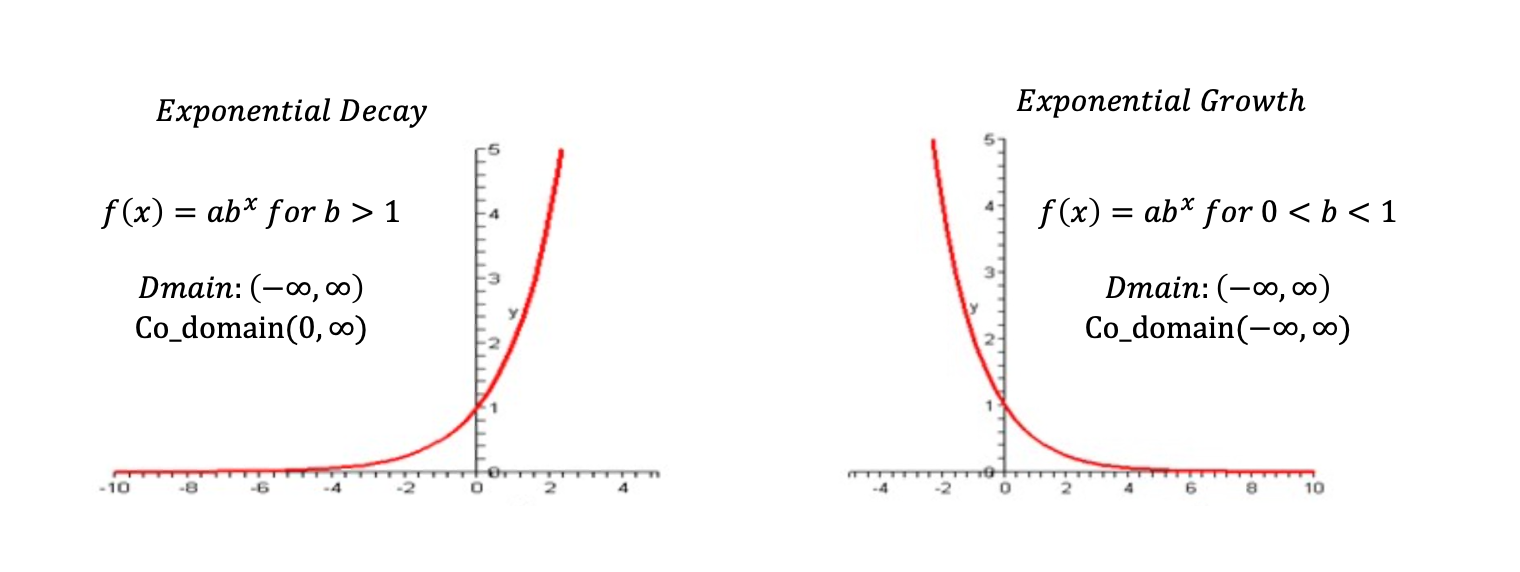
\includegraphics[width=12cm]{images/Function.png}
    \caption{The graph representation of $f(x) = ab^x$}
    \label{fig:my_label}
\end{figure}

\subsection{Context of Use Model}
The context of use model for the exponential function calculator\cite{zelen1966application}\cite{lebanon2001boosting} is represented by the UML Class Diagram as Figure \ref{fig:context}.
\begin{figure}[h]
    \centering
    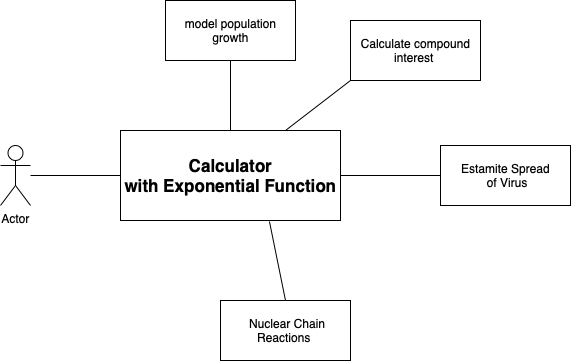
\includegraphics[width=10cm]{images/Context_diagram.png}
    \caption{The Context Diagram for exponential function calculator}
    \label{fig:context}
\end{figure}

\begin{enumerate}
\item User: Users who use the calculator to get the output of $ab^x$ with the input x.
\item Task: Calculate the output of $ab^x$ with the input $x$ and show the result to the user.
\item
Environment:
\begin{itemize}
\item Technical environment:
The power function of the used calculator. This calculator can't be used without power function.
\item Non-technical environment:
The location of where the user use this calculator.
\end{itemize}
\end{enumerate}

\section{Project Requirements}\label{problem2}
This section presents the assumptions and requirements\cite{iso2018ieee} for implementing $f(x)=ab^x$.
\subsection{Assumptions}
\begin{enumerate}
    \item The Function will accept only real numbers as inputs.
    \item The Function will be able to handle entry value of double-precision floating-point.
\end{enumerate}

\subsection{Requirements}
\begin{center}
    \begin{tabular}{|p{3cm}|p{11cm}| }
    \hline
    \textbf{Identification} &  FR1 \\ \hline 
    \textbf{Type} & Functional Requirement\\ \hline
    \textbf{Version No.} &  1.0 \\ \hline 
    \textbf{Owner} &  Yun Ni \\ \hline 
    \textbf{Priority} & High  \\ \hline
    \textbf{Difficulty} & Medium  \\ \hline
    \textbf{Description} & System needs to take inputs $x, a, b$ to give an output of $ab^x$. Besides, needs to define the constrains that $a\neq0, b > 0$. Because, when $a=0$ the function will be simplified to $y = f(x) = 0$. \\ \hline
\end{tabular}
\end{center}

\begin{center}
    \begin{tabular}{|p{3cm}|p{11cm}| }
    \hline
    \textbf{Identification} &  FR2 \\ \hline 
    \textbf{Type} & Functional Requirement\\ \hline 
    \textbf{Version No.} &  1.0 \\ \hline 
    \textbf{Owner} &  Yun Ni \\ \hline 
    \textbf{Priority} & High  \\ \hline
    \textbf{Difficulty} & Medium  \\ \hline
    \textbf{Description} & Function $ab^x$ does not depend on any other functions like built-in or library functions.\\ \hline
\end{tabular}
\end{center}

\begin{center}
    \begin{tabular}{|p{3cm}|p{11cm}| }
    \hline
    \textbf{Identification} &  FR3 \\ \hline 
    \textbf{Type} & Functional Requirement\\ \hline
    \textbf{Version No.} &  1.0 \\ \hline 
    \textbf{Owner} &  Yun Ni \\ \hline 
    \textbf{Priority} & High  \\ \hline
    \textbf{Difficulty} & Medium  \\ \hline
    \textbf{Description} & Users can give an input from all real numbers for $x$.\\ \hline
\end{tabular}
\end{center}

\begin{center}
    \begin{tabular}{|p{3cm}|p{11cm}| }
    \hline
    \textbf{Identification} &  FR4 \\ \hline 
    \textbf{Type} & Functional Requirement\\ \hline 
    \textbf{Version No.} &  1.0 \\ \hline 
    \textbf{Owner} &  Yun Ni \\ \hline 
    \textbf{Priority} & High  \\ \hline
    \textbf{Difficulty} & Easy  \\ \hline
    \textbf{Description} & When users give other inputs than a number like a string, the system should not accept and should show the exception properly.\\ \hline
\end{tabular}
\end{center}

\begin{center}
    \begin{tabular}{|p{3cm}|p{11cm}| }
    \hline
    \textbf{Identification} &  FR5 \\ \hline 
    \textbf{Type} & Functional Requirement\\ \hline
    \textbf{Version No.} &  1.0 \\ \hline 
    \textbf{Owner} &  Yun Ni \\ \hline 
    \textbf{Priority} & High  \\ \hline
    \textbf{Difficulty} & Easy  \\ \hline
    \textbf{Description} & When users give inputs does not specify all there inputs like $a, b, x$, the system should not accept and throw an error.\\ \hline
\end{tabular}
\end{center}

\begin{center}
    \begin{tabular}{|p{3cm}|p{11cm}| }
    \hline
    \textbf{Identification} &  FR6 \\ \hline 
    \textbf{Type} & Functional Requirement\\ \hline
    \textbf{Version No.} &  1.0 \\ \hline 
    \textbf{Owner} &  Yun Ni \\ \hline 
    \textbf{Priority} & High  \\ \hline
    \textbf{Difficulty} & Easy  \\ \hline
    \textbf{Description} &Ensure the accuracy of decimal operations to the power of decimals.\\ \hline
\end{tabular}
\end{center}

\begin{center}
    \begin{tabular}{|p{3cm}|p{11cm}| }
    \hline
    \textbf{Identification} &  NFR1 \\ \hline 
    \textbf{Type} & Non-Functional Requirement\\ \hline
    \textbf{Version No.} &  1.0 \\ \hline 
    \textbf{Owner} &  Yun Ni \\ \hline 
    \textbf{Priority} & High  \\ \hline
    \textbf{Difficulty} & Easy  \\ \hline
    \textbf{Description} & Users need to have the Java environment to use the project.\\ \hline
\end{tabular}
\end{center}

\section{Algorithm}\label{problem3}
This section presents the pseudo-code and algorithm for implementing $f(x)=ab^x$.
\subsection{Mind map}

\begin{figure}[h]
    \centering
    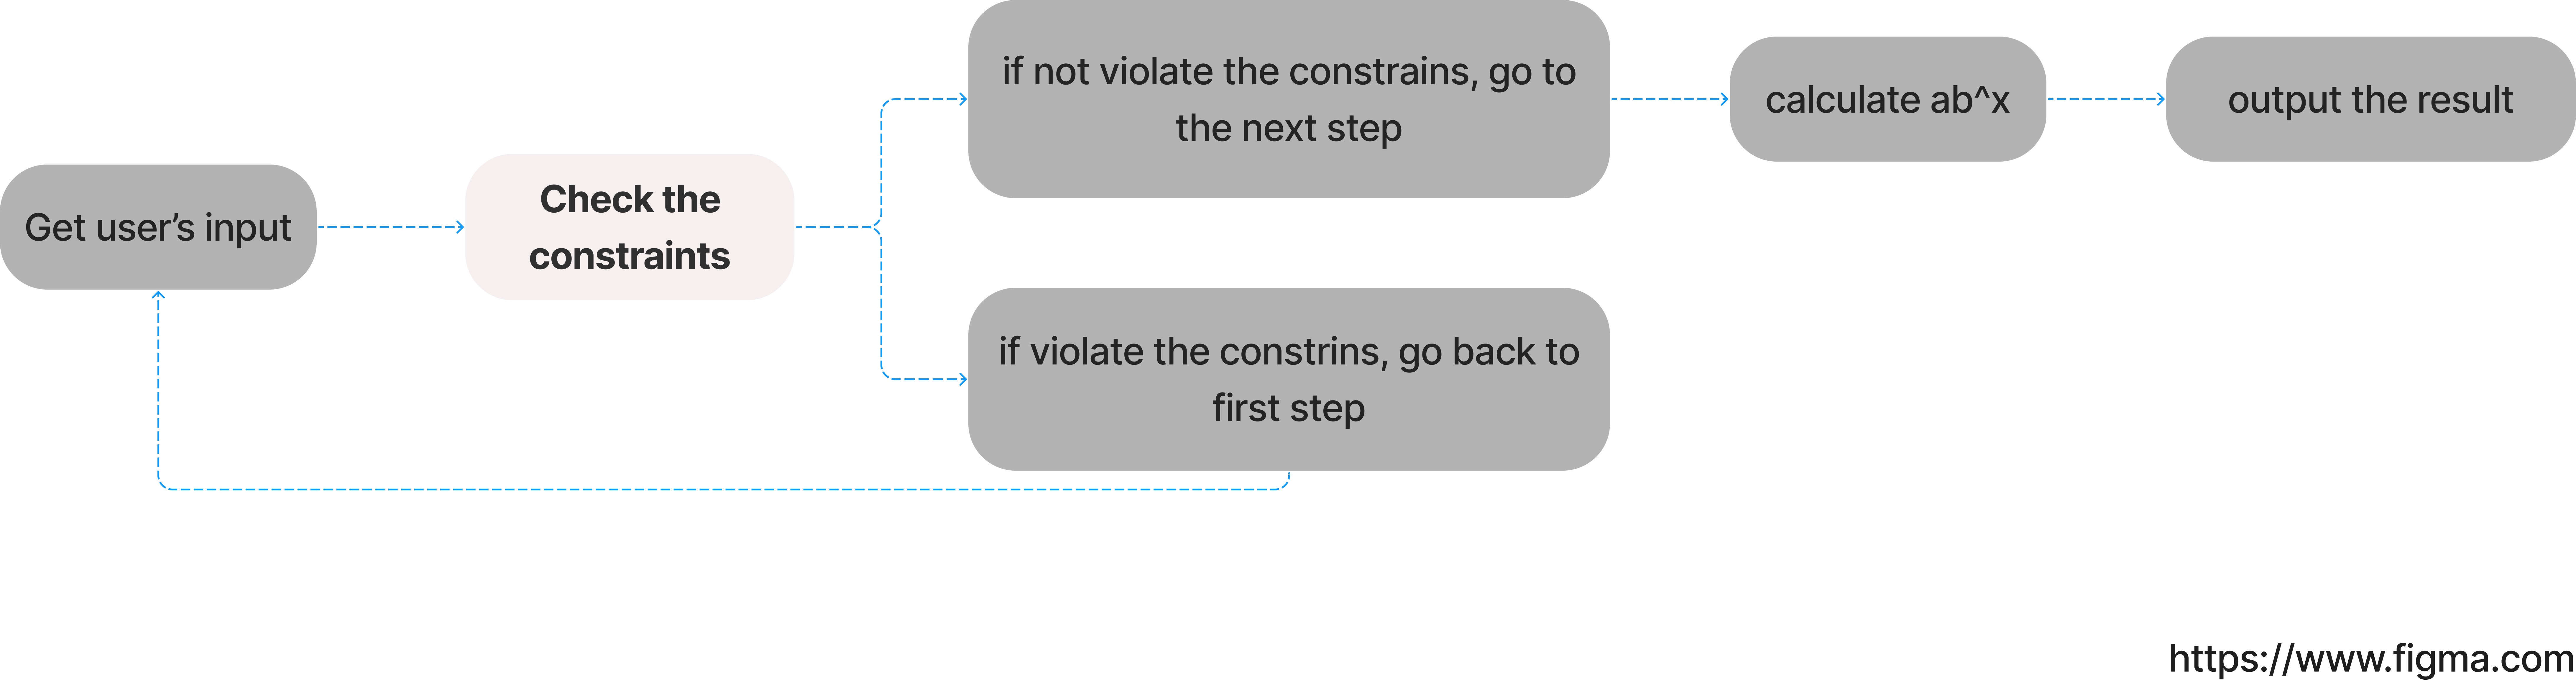
\includegraphics[width=13cm]{images/mindmap.jpeg}
    \caption{The mind map of algorithm design}
    \label{fig:mind}
\end{figure}

\subsection{Algorithm 1: Iterative}
The interactive algorithm can execute the steps in number of iterations, using the loop. We can track the result in a variable called prod, which is initially set to 1 and then use loop from 1 to x number of times. By incriminating by one on each iteration, we multiply prod by b. At the end of the loop value of prod is equal to $b^x$ then return the result of $a * prod$\cite{xu2015application}.

\begin{algorithm}
  \caption{Iterative algorithm for calculating $f(x) = ab^x$}
  \begin{algorithmic}[1]
  \Require $a \neq 0$ and $b > 0$ and $b \neq 1$ 
    \Function\textbf{\textbf{exponent\_iterative(a,b,x)}}\\
    \textbf{in: }double number x, a, b\\
    \textbf{out: }double number prod
    \State $prod \gets 1$
    \State $temp \gets 1$
    \For{\texttt{$temp \leq x$}}
        \qquad \State $prod \leftarrow prod*b$
        \qquad \State $temp \leftarrow temp+1$
    \EndFor
    \State $prod \gets prod*a$
    \State return $prod$
    \EndFunction
  \end{algorithmic}
\end{algorithm}

\begin{center}
\begin{tabular}{|p{7cm}|p{7cm}|}
\hline
     \textbf{Advantages} & \textbf{Disadvantages}\\ \hline
     Easy to implement, since it uses looping structure. & If the condition fails, the iteration terminates the execution of the program.\\ \hline
     Tracing the iterative algorithm is easy. & It is not very efficient in terms of time since the time complexity is $O(n)$ for a larger input\cite{xu2015application}. \\ \hline
     Could avoid memory overflow of input. & Can not calculate decimal inputs properly in this case.\\ \hline
\end{tabular}
\end{center}

\subsection{Algorithm 2: Recursive}
A recursive function calls by itself during the execution of the program, until the base conditions are met\cite{haberman2002case}. By defining a helper function called exponent\_helper which calculates $b^x$ in different conditions. With the helper function, we multiply the result to the value of input $a$ and return it to the user.

\begin{algorithm}
  \caption{Recursive algorithm for calculating $f(x) = ab^x$}
  \begin{algorithmic}[1]
  \Require $a \neq 0$ and $b > 0$ and $b \neq 1$ 
   \Function\textbf{\textbf{exponent\_recursive(a,b,x)}}\\
    \textbf{in: }double number x, a, b\\
    \textbf{out: }double number prod
    \State $power \gets exponent\_helper(b,x)$
    \State $prod \gets power * a$
    \State return $prod$
    \EndFunction
  \end{algorithmic}
\end{algorithm}

\begin{algorithm}
  \begin{algorithmic}[1]
   \Function\textbf{\textbf{exponent\_helper(b,x)}}\\
   \textbf{in: }number x, b\\
   \textbf{out: }double number prod
   \If{$x < 0$}
   \State $b \gets 1.0 / b$
   \State $x \gets -x$ 
   \State return $exponent\_helper(b, x)$ 
   \ElsIf{$x = 0$}
     \State return $1.0$
   \ElsIf{ $x = 1$}
    \State return $b$
   \ElsIf{$x \mod  2 = 0$}
    \State $b \gets b * b$ 
    \State $x \gets x / 2$ 
    \State return $exponent\_helper(b, x)$
    \Else
    \State $b \gets b * b$ 
    \State $x \gets x - 1$ 
    \State $x \gets x / 2$ 
    \State return $exponent\_helper(b, x)$
    \EndIf 
   \EndFunction
  \end{algorithmic}
\end{algorithm}

\begin{center}
\begin{tabular}{|p{7cm}|p{7cm}|}
\hline
     \textbf{Advantages} & \textbf{Disadvantages}\\ \hline
     The time complexity of the defined recursive algorithms above is $O(\log n)$. & Recursive algorithm is not easy to debug since it calls itself.\\ \hline
     Recursive algorithms is easier to maintain than loop\cite{karigl1981recursive}. & Recursive algorithm needs the system continuously allocates memory, might lead stack overflow\cite{haberman2002case} \\ \hline
      & Can not calculate decimal inputs properly in this case.\\ \hline
\end{tabular}
\end{center}

\subsection{Algorithm 3: Taylor Series for calculating $f(x) = ab^x$}
For calculating the exponential function $f(x) = ab^x$ more properly, we can use Taylor Series algorithm. When $x$ is a decimal, Taylor Series can calculate $\ln(x)$ and $e^x$ with a high precision, since the formula can be changed to $b^x = e^{b\ln b}$. When $x$ is an integer, if $x$ is an even number, $b^x$ can be decomposed to $(b^2) (x/2)$; if $x$ is an odd number, $b^x$ can be decomposed to $b\cdot ((b^2) ((x-1)/2)$. And then continue to decompose until the exponent part is equal to one\cite{abad2012algorithm}.

\begin{algorithm}
\caption{Exponentiation by Taylor Series\cite{Anu:Stack_Overflow}}\label{exp1}
\begin{algorithmic}[1]
\Require $a \neq 0$ and $b > 0$ and $b \neq 1$ 
\Function{logarithm}{$n$}
\State $sum\gets 0$
\While{$n > 1$}
    \State $n\gets n/e$\Comment{e is a constant approximately equal to 2.71828}
    \State $x \gets x + 1 $
\EndWhile \\
\Return $x$
\EndFunction

\Function{exponential}{$b$}
\State $sum\gets 1$
\State $n\gets 10$
\For{$i\gets n-1$, 1}
\State $sum\gets 1+ b * sum / i$
\EndFor \\
\Return $sum$
\EndFunction

\State $\log b \gets $\Call{logarithm}{$b$}
\State $result \gets $\Call{exponential}{$x* \log b$}
\State $result \gets $\Call{$a\cdot$}{$result$}
\end{algorithmic}
\end{algorithm}

\begin{center}
    \begin{tabular}{|p{7cm}|p{7cm}|}\hline
        \textbf{Advantages} & \textbf{Disadvantages}\\\hline
        The Taylor Series is very useful for derivations and can calculate even the most complex functions. & The algorithm could be very complex with deriving.\\\hline The Taylor Series can be used to get theoretical error bounds and estimate the value of any input\cite{hariharan2010comparative}.  & The expansion point might lead truncation errors.\\\hline
    \end{tabular}
\end{center}
\subsection{Conclusion}
For a function, the accuracy is the most significant factor, since a wrong output is worse than a blank. The iterative and recursion algorithms can not calculate the decimal part of $f(x) = ab^x$ with high precision, therefore, my decision is to use Taylor Series algorithm and the sub-function of the recursive algorithm to implement the project. It  runs more efficiently and provide results with high accuracy.

\section{Code Implementation}
\subsection{Debugger}
IntelliJ has a standard build-in debugger which allows the program to open in debug mode. It supports both step by step debugging, break point, check points and multiple views which enhance the experience of debugging.

\begin{figure}[h]
    \centering
    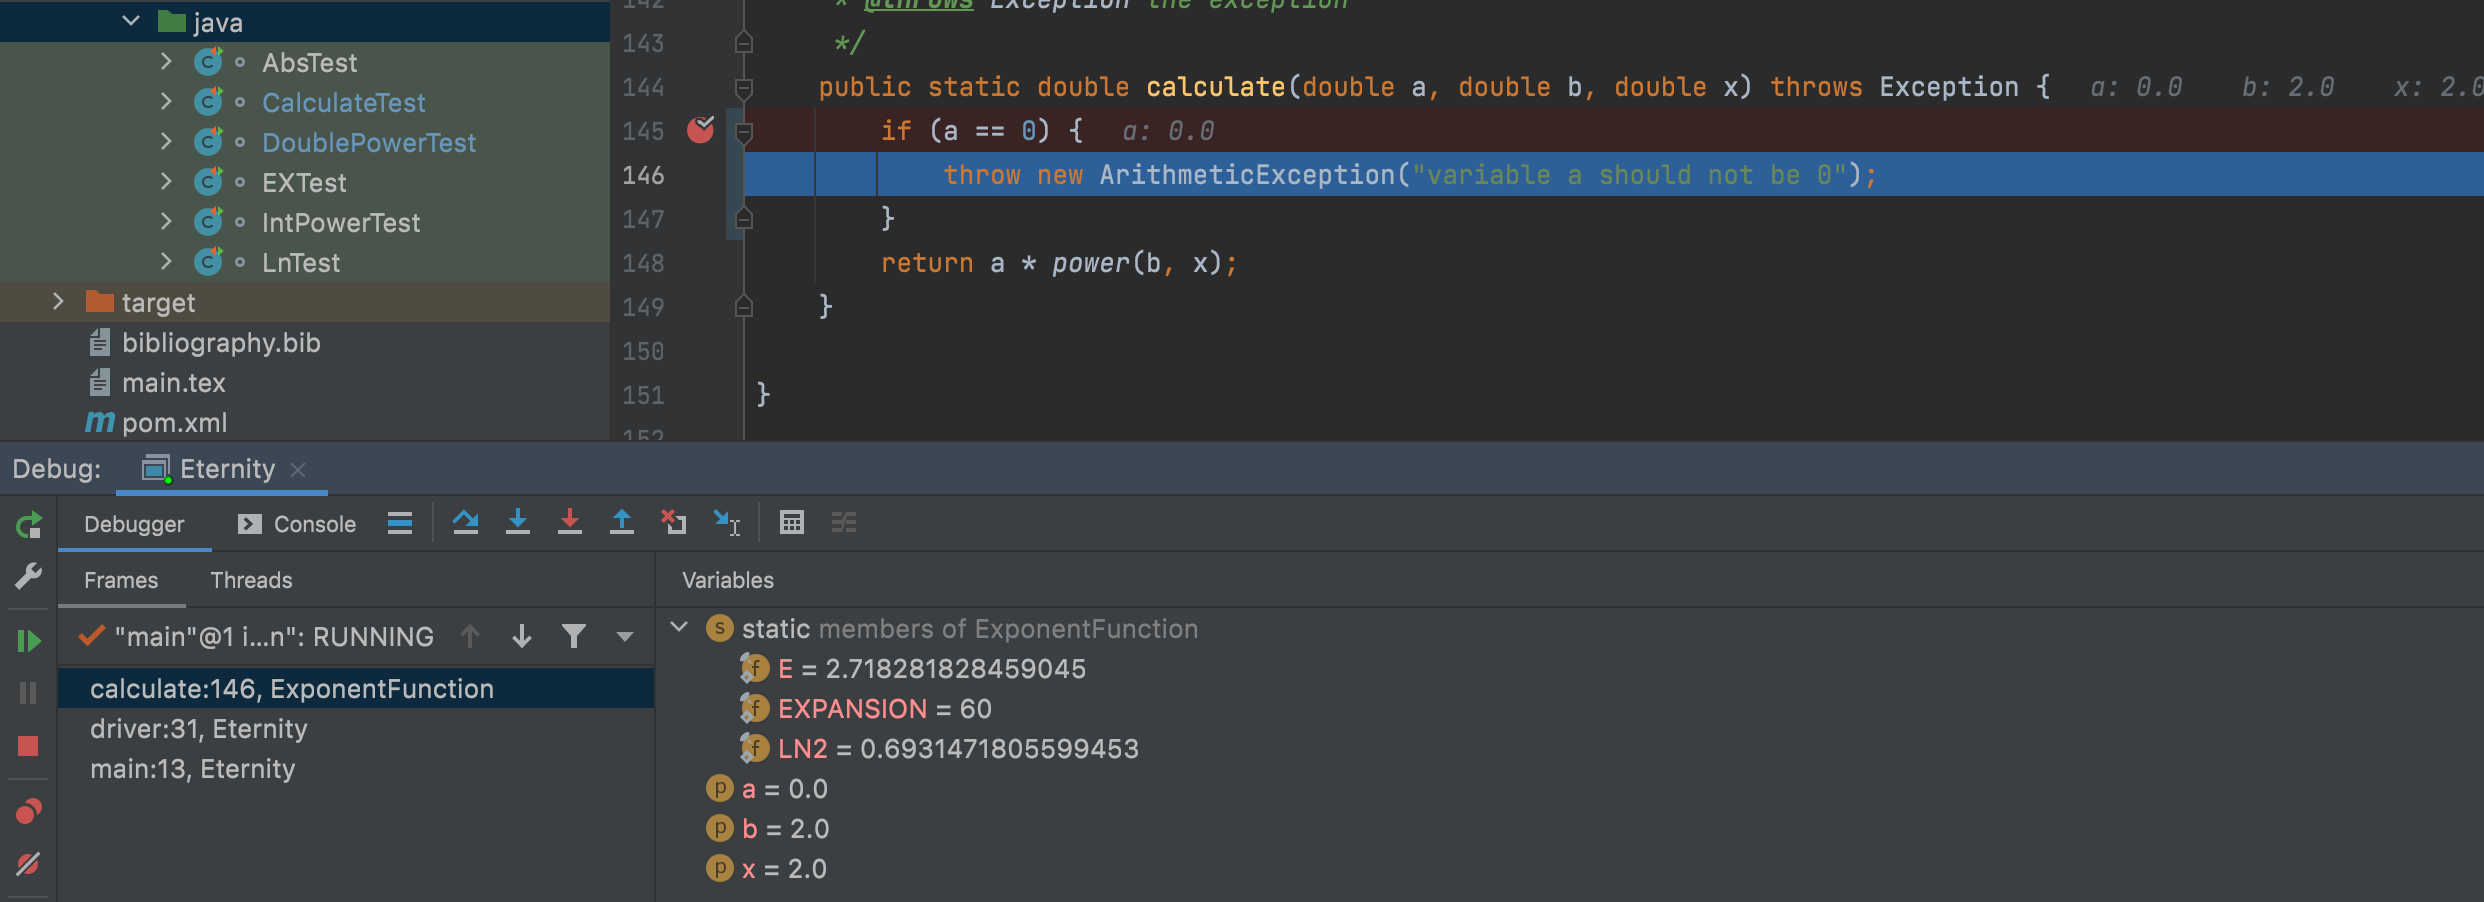
\includegraphics[width=15cm]{images/debugger.png}
    \caption{The snapshot of the debugger in IntelliJ}
    \label{fig:debugger}
\end{figure}

\subsubsection{Advantages of the Debugger}
\begin{center}
    \begin{itemize}
        \item As a build-in tool, it can be easily accessed by users. Users can create various kinds of breakpoints, such as conditional breakpoints to trace the source code.
        \item Users can stop execution at a given point to investigate where it goes and what the values are.
        \item The hot swapping function allows users to insert minor changes in the code without shutting down the process which is convenient.\cite{Anu:StackExchange}
    \end{itemize}
\end{center}

\subsubsection{Disadvantages of the Debugger}
\begin{center}
    \begin{itemize}
        \item For the multi-threading programs, the debugger tool in IntelliJ could not work efficient.
        \item The debugger can not solve the bad code or correct the code.
        \item The IntelliJ may run into bad state and have to clear the caches and restart the IDE to go through the build-clean-build to fix it.
    \end{itemize}
\end{center}

\subsection{The Quality Attributes}
The quality attributes assessed while implementing the source code and program are:
\begin{center}
    \begin{itemize}
        \item \textbf{Efficiency}: In order to achieve efficiency, the primitive data types are used instead of using the user-defined data type. Therefore, the output is generated in the order of milliseconds.
        \item \textbf{Portability}: With the executable jar file, users can use the program without any difficulties which could increase the portability.
        \item \textbf{Maintainability}: Giving the simple and understandable names to variables could improve the maintainability. If there is an error in the function, I can locate the errors by their names. Besides, the core logic and the error handling have been properly implemented with comments.
        \item \textbf{Correctness}: For the function $y = ab^x$, when x is an integer, the result can get easily by a loop or a recursion. When x is a decimal, the loop could generate incorrect result. To improve the accuracy, the Taylor Expansion is used to get the similar value of the $b^x$, then multiply by $a$ which could reduce the error.
        \item \textbf{Robustness}: My program supports for the error handling, exceptions and thrown to handle errors. Therefore, the program will not crash and notify the users with appropriate error messages.
        \item \textbf{Usability}: By providing the textual user interface for the project, users can use the calculator easily.
    \end{itemize}
\end{center}

\subsection{Checkstyle}
CheckStyle for java can scan the source code and point out coding issues that the code might have missed or might lead to problems.
It can also help improve the Java Coding because we have to investigate and decide if this is a problem or not. I am using Google Checkstyle in the program like in Figure\ref{fig:Checkstyle} and Figure\ref{fig:Checkstyle2}.
\begin{figure}[p]
    \centering
    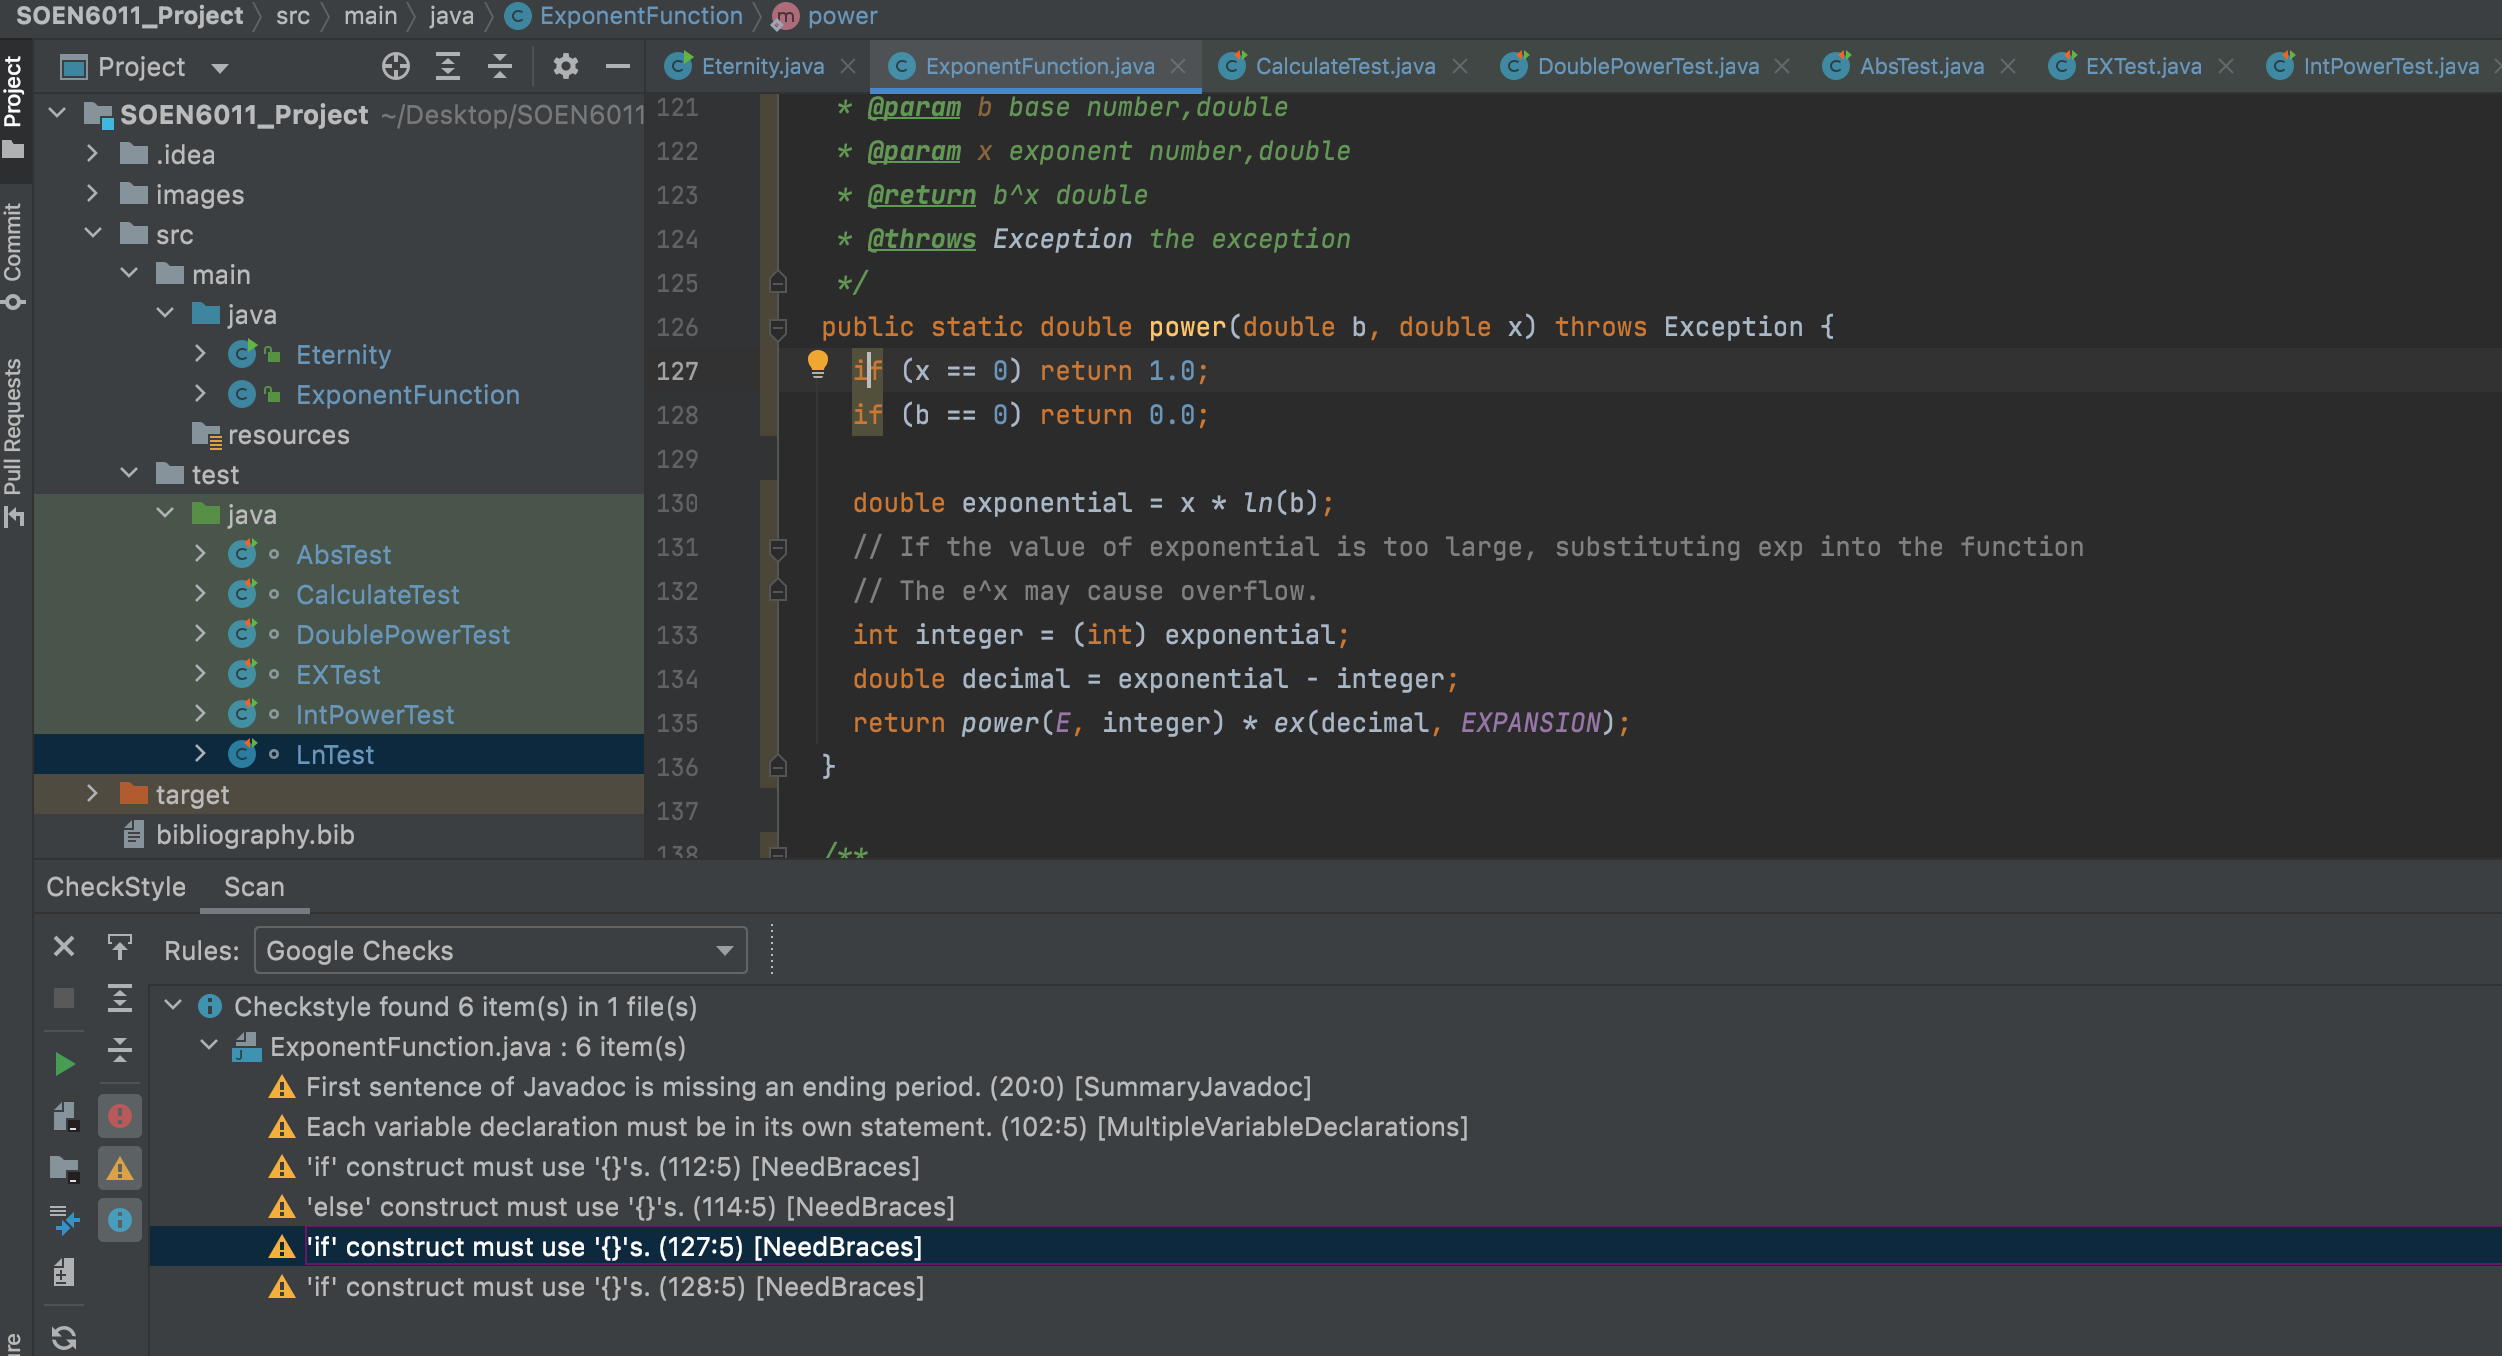
\includegraphics[width=15cm]{images/checkstyle.png}
    \caption{The snapshots of the Checkstyle}
    \label{fig:Checkstyle}
\end{figure}

\begin{figure}[p]
    \centering
    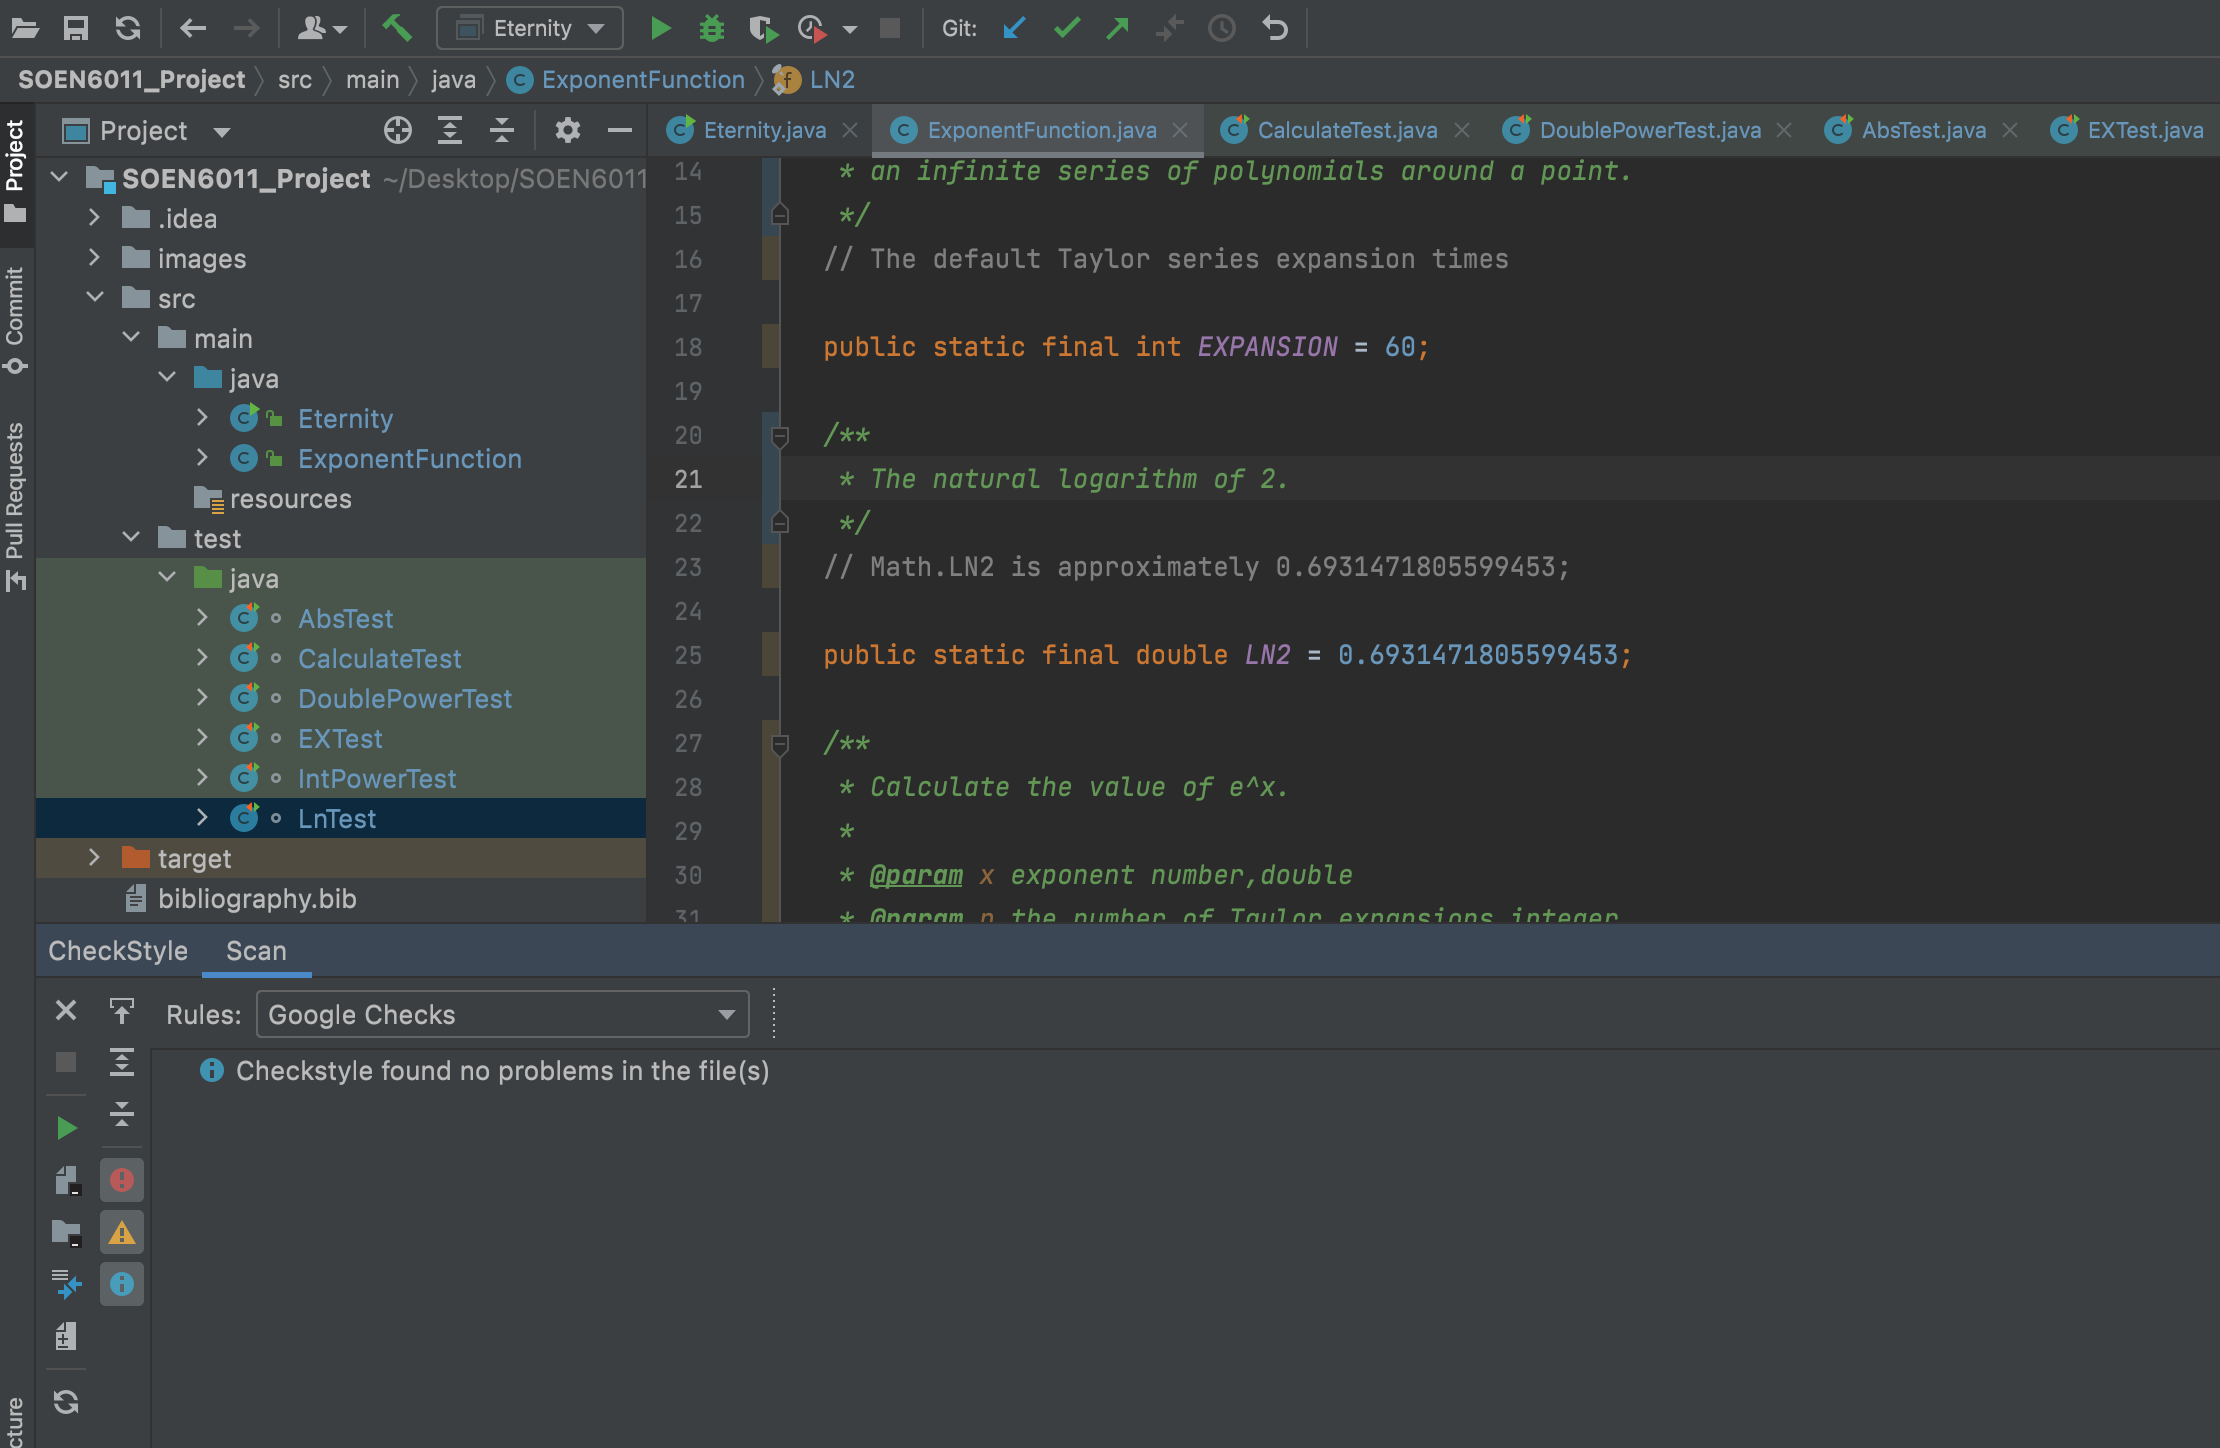
\includegraphics[width=15cm]{images/check2.png}
    \caption{The snapshots of the Checkstyle}
    \label{fig:Checkstyle2}
\end{figure}

\subsubsection{Advantages of the Checkstyle}
\begin{center}
    \begin{itemize}
        \item It is a convenient external plug and can be installed directly in the IntelliJ IDEA. 
        \item It can check the layout and the formatting issue.
        \item It gives developers the ability to customize their own rules for checking.
    \end{itemize}
\end{center}

\subsubsection{Disadvantages of the Checkstyle}
\begin{center}
    \begin{itemize}
        \item It is limited to only the code beautification. No logic checks at present.
        \item There is no modification function after checking. Developers need to modify the problems one by one.
    \end{itemize}
\end{center}

\section{Unit Test}
Junit is a unit testing framework for Java programming language and has been import to the development of test-driven developments. In this project, Junit4 has been used to write the test cases.
\subsection{Mapping Requirements with Test Cases}
\begin{center}
\begin{tabular}{|p{5cm}|p{10cm}|}
\hline
     \textbf{Requirement Identifier} & \textbf{Test Cases}\\ \hline
      \textbf{FR1} & exceptionCalculate(), negativeCalculate()\\ \hline
      \textbf{FR2} & absZero(), lnZero(), zeroPowerZero() \\ \hline
      \textbf{FR3} & zeroPowerZero(), zeroPowerRationalNumber() \\ \hline
      \textbf{FR4} & lnOfNegativeValues(), lnZero() \\ \hline
      \textbf{FR5} & ePowerRealNumber(), exceptionCalculate()\\\hline
      \textbf{FR6} & positiveNumberPowerZero(), positiveNumberPowerOne()\\ \hline
\end{tabular}
\end{center}

\subsection{Test Cases}
\begin{center}
    \begin{tabular}{|p{4cm}|p{11cm}| }
    \hline
    \textbf{Test Case ID} & Test Case 1\\ \hline 
    \textbf{Class Name} &  AbsTest\\ \hline 
    \textbf{Method Name} & absZero(), absPositive(), absNegative()\\ \hline 
    \textbf{Description} & Testing the absolute value function\\ \hline
    \textbf{Input(s)} & 0; 5; -5\\ \hline
    \textbf{Expected Output(s)} & 0; 5; 5\\ \hline
    \textbf{Actual Output(s)} & 0; 5; 5\\ \hline
    \textbf{Test Result} & Passed\\ \hline
\end{tabular}
\end{center}

\begin{center}
    \begin{tabular}{|p{4cm}|p{11cm}| }
    \hline
    \textbf{Test Case ID} & Test Case 2\\ \hline 
    \textbf{Class Name} &  EXTest\\ \hline 
    \textbf{Method Name} & ePowerZero(), ePowerPositive(), ePowerNegative(),  ePowerRealNumber() \\ \hline 
    \textbf{Description} & Testing $e^x$ function with expansion equals 60\\ \hline
    \textbf{Input(s)} & 0; 10; -10; 2.71818\\ \hline
    \textbf{Expected Output(s)} & 1; 22026.46; 4.53; 15.15\\ \hline
    \textbf{Actual Output(s)} & 0; 5; 5\\ \hline
    \textbf{Test Result} & Passed\\ \hline
\end{tabular}
\end{center}

\begin{center}
    \begin{tabular}{|p{4cm}|p{11cm}| }
    \hline
    \textbf{Test Case ID} & Test Case 3\\ \hline 
    \textbf{Class Name} &  LnTest\\ \hline 
    \textbf{Method Name} & lnZero(), lnOfPositiveValues(), lnOfNegativeValues() \\ \hline 
    \textbf{Description} & Testing $ln^x$ function \\ \hline
    \textbf{Input(s)} & 0; 1; 53; -2\\ \hline
    \textbf{Expected Output(s)} & throw exception; 0; 3.97; throw exception\\ \hline
    \textbf{Actual Output(s)} &throw exception; 0; 3.97; throw exception\\ \hline
    \textbf{Test Result} & Passed\\ \hline
\end{tabular}
\end{center}

\begin{center}
    \begin{tabular}{|p{4cm}|p{11cm}| }
    \hline
    \textbf{Test Case ID} & Test Case 4\\ \hline 
    \textbf{Class Name} &  IntPowerTest\\ \hline 
    \textbf{Method Name} & zeroPowerZero(), positiveNumberPowerZero(), negativeNumberPowerPositiveEvenNumber(), negativeNumberPowerNegativeNumber(), positiveNumberPowerOne() \\ \hline 
    \textbf{Description} & Testing $b^x$ function with input with integers\\ \hline
    \textbf{Input(s)} & (0, 0); (-4, 0); (-3, 4); (-5, -9); (7, 1)\\ \hline
    \textbf{Expected Output(s)} & 1; 1; 81; -5.12E-7; 7\\ \hline
    \textbf{Actual Output(s)} & 1; 1; 81; -5.12E-7; 7\\ \hline
    \textbf{Test Result} & Passed\\ \hline
\end{tabular}
\end{center}

\begin{center}
    \begin{tabular}{|p{4cm}|p{11cm}| }
    \hline
    \textbf{Test Case ID} & Test Case 5\\ \hline 
    \textbf{Class Name} & DoublePowerTest\\ \hline 
    \textbf{Method Name} & zeroPowerZero(),  positiveNumberPowerZero(), negativeNumberPowerNegativeNumber(), positiveNumberPowerZero()  \\ \hline 
    \textbf{Description} & Testing $b^x$ function with inputs type double \\ \hline
    \textbf{Input(s)} & (0.0, 0.0); (7.0, 1.0); (5.5, -9.6); (0.0, 5.8)\\  \hline
    \textbf{Expected Output(s)} & 1.0; 6.99; throw error; 0.0 \\ \hline
    \textbf{Actual Output(s)} & 1.0; 6.99; throw error; 0.0 \\ \hline
    \textbf{Test Result} & Passed\\ \hline
\end{tabular}
\end{center}

\begin{center}
    \begin{tabular}{|p{4cm}|p{11cm}| }
    \hline
    \textbf{Test Case ID} & Test Case 6\\ \hline 
    \textbf{Class Name} & CalculateTest\\ \hline 
    \textbf{Method Name} & integerCalculate(); positiveCalculate(); exceptionCalculate(); positiveCalculate()\\ \hline 
    \textbf{Description} & Testing $ab^x$ function with inputs\\ \hline
    \textbf{Input(s)} & (5, 3, 10); (2, 3.6, -2.3); (0, 2, 2); (6.3, 1.2, 1.3)\\  \hline
    \textbf{Expected Output(s)} & 295245; 0.10508343093; throw exception; 8.36526215004 \\ \hline
    \textbf{Actual Output(s)} & 295245; 0.10508343093; throw exception; 8.36526215004 \\ \hline
    \textbf{Test Result} & Passed\\ \hline
\end{tabular}
\end{center}

\section{Conclusion}
Building a project, it is necessary to have an explicit scoping and separate each functional module. With this project, I understand the process of each stage. Even this project is a small scale, I met each stage of the project development process and gained the knowledge with the various implementation methods and tools which can be used officially in the real industry.

\newpage
\bibliographystyle{plain}
\bibliography{bibliography.bib}
\end{document}